% !TeX root = main.tex
% !TeX program = xelatex
\section{Motivation from biology}\label{motivation-from-biology}

AI as a field often draws inspiration from biology.

Recent discoveries point that there is at least some intelligence on different levels of organization.

Molecular networks have memory including pavlovian conditioning, associative learning etc.

Also there is no large difference between neural cells and somatic cells. Somatic cells exhibit learning, problem solving, they also use electricity for communication.

Some notable examples of plasticity and problem solving:

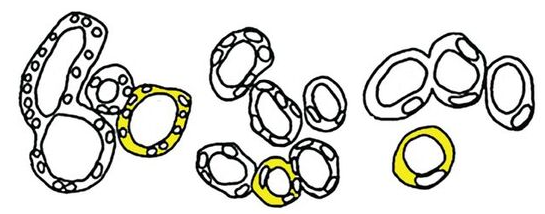
\includegraphics[width=5.67708in,height=2.22917in]{figures/image8.png}

\hl{Kidney tubules in the newt are made with a constant size, whereas cell size can vary drastically under polyploidy. The same shape achieved through different molecular mechanisms: cell to cell communication vs cytoskeleton bending.}

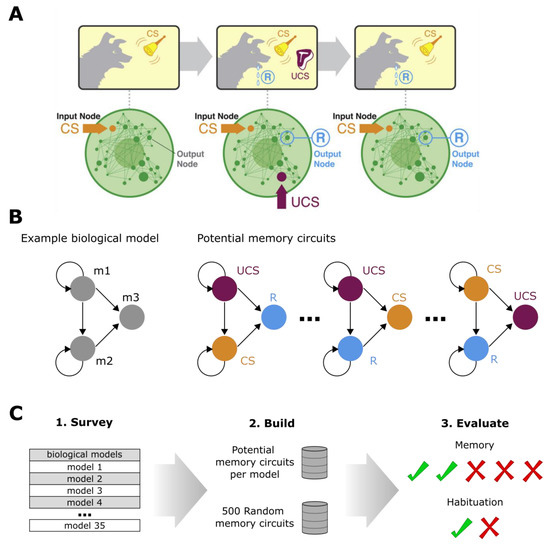
\includegraphics[width=5.72917in,height=5.66667in]{figures/image3.png}

\hl{Classical conditioning in biological network, for example drug-drug conditioning}

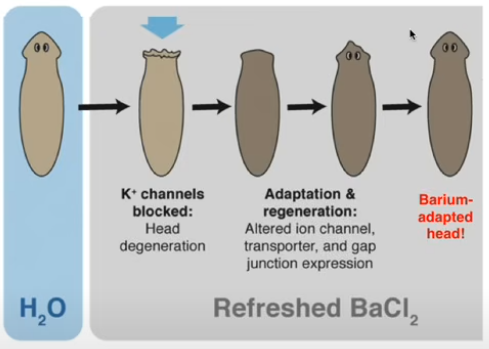
\includegraphics[width=5.09375in,height=3.63542in]{figures/image7.png}

\hl{Adaptation of neurons in planaria to barium chloride. After exposure to BaCL2 neurons in planaria's head die off. New head has resistant neurons. It's unlikely that planaria has ever been exposed to BaCL2 before.}

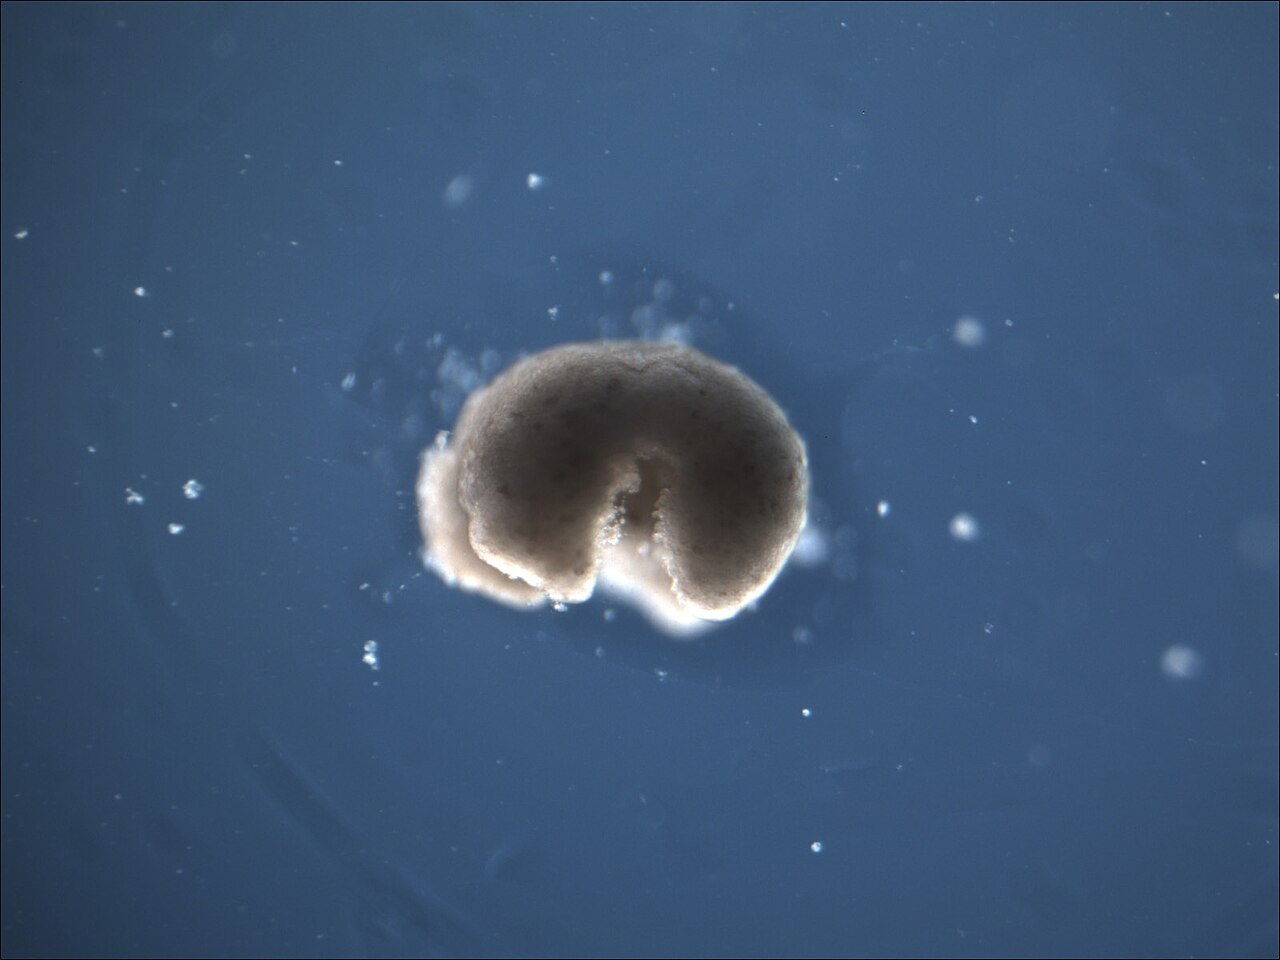
\includegraphics[width=6.59299in,height=4.94474in]{figures/image11.png}

\hl{Xenobots - small, self-organizing robots made from frog embryonic cells (Xenopus laevis). This one is made of skin and cardiac cells.}

\hl{But perhaps the most striking and important case is cancer plasticity. Tumors switch between metabolic pathways (e.g., glycolysis to oxidative phosphorylation) to survive fluctuating conditions, a form of tissue-level adaptability.}

\section{Learning hierarchy}\label{learning-hierarchy}

\hl{We can roughly sort different learning types from more simple to more advanced forms, that appeared later in evolutionary history:}

\begin{enumerate}
\def\labelenumi{\arabic{enumi}.}
\item
  Non-associative learning
\end{enumerate}

Habituation - decrease of response to non-harmful repeated stimulus

Sensitization - increase of response after exposure to strong or harmful stimulus.

\begin{enumerate}
\def\labelenumi{\arabic{enumi}.}
\setcounter{enumi}{1}
\item
  Associative (Classical \&)
\end{enumerate}

Classical conditioning: Response is modified by its consequences (reward, punishment).

Operant Conditioning: Trial and error learning.

\begin{enumerate}
\def\labelenumi{\arabic{enumi}.}
\setcounter{enumi}{2}
\item
  Observational/Social Learning/play and metacognition
\end{enumerate}

\begin{quote}
Metacognition. This includes capacity to model agent's own understanding e.g. being uncertain, seek more information, being able to assess own likelihood of error.

Spatial Learning \& Navigation

Insightful Problem Solving, probably based on some internal modelling as opposed to trial and error.

Teaching \& Pedagogy
\end{quote}

\begin{enumerate}
\def\labelenumi{\arabic{enumi}.}
\setcounter{enumi}{3}
\item
  Cumulative Culture:
\end{enumerate}

\begin{quote}
Cultural learning over generations, learning from purely symbolic input e.g. reading instructions.
\end{quote}

Level 2 and Level 3 learning types can be observed already in insects. Bumblebee for example would play with appropriately sized balls without any external reward from only intrinsic motivation. Another example is Portia spiders which employ a sophisticated hunting strategy involving mimicry, detours, and ambush tactics when hunting on other spiders. Portia often attacks other spiders in their own web, so it has to be clever. Sometimes it will literally lure the prey by mimicking vibrations of an insect being stuck. It has been reported that Portia can learn to hunt a new, never seen before spider by trial and error.

Portia is a very good example since it has a very small brain. Bumblebees have approximately 950k - 1 mln neurons vs Portia around 100k.

From observations we can conclude that it has:

\textbf{Internal Representation:} The ability to take a detour where the prey is out of sight for extended periods implies the spider is not just reacting to the prey\textquotesingle s presence. It must be operating from a stored representation of the environment and the prey\textquotesingle s location within it.

\textbf{Object Permanence and Spatial Memory:} Portia\textquotesingle s behavior indicates it has a grasp of object permanence (knowing the prey still exists even when it can\textquotesingle t be seen) and strong spatial memory to navigate the planned route.

\textbf{Systematic Scanning:} The process of systematically scanning its surroundings before a hunt is interpreted as the spider building a detailed mental map of the area, which it then uses to execute its plan.

\textbf{Expectancy Violation:} When a spider takes a wrong turn and reaches a dead end, it has been observed to pause in a way that suggests confusion. This implies it had an expectation of what it should find, based on its internal model, and that expectation was violated.

Also there is growing evidence about tool use by insects. Image 5 shows the experiment: researchers gave hungry ants containers with sugar water. Researchers then altered the surface tension of the sugar water by adding surfactant. When surfactant concentrations were over 0.05\%, representing considerable drowning risk, ants were observed building the sand structures to syphon sugar water out of the container. These structures were never observed when ants foraged in containers of pure sugar water, indicating an adaptable approach to this novel tool use.

\hl{}

\href{https://www.facebook.com/DailyPlanet/videos/teaching-bees-to-play-soccer/2683370568353442/}{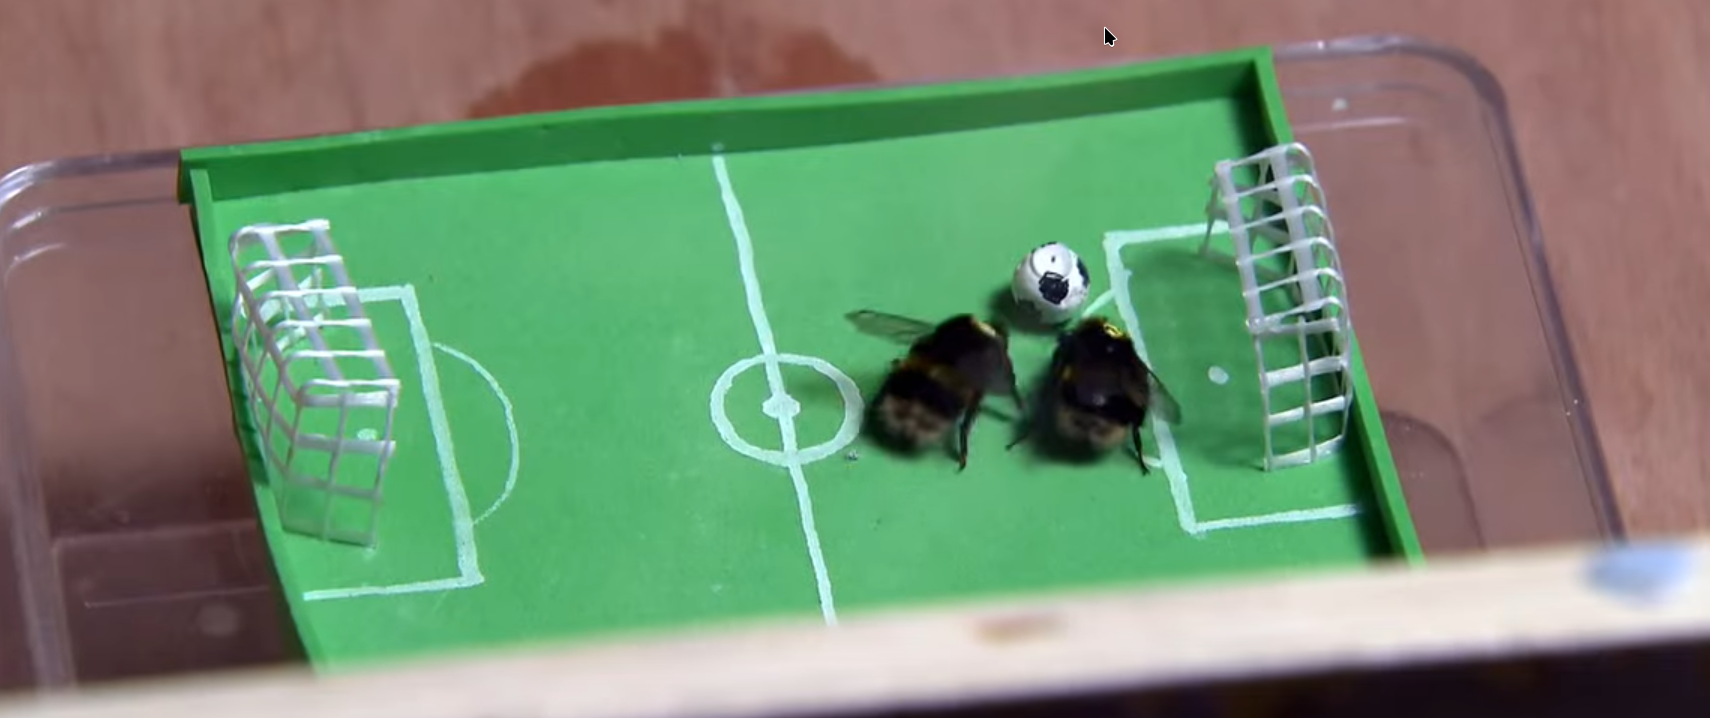
\includegraphics[width=2.91196in,height=1.2265in]{figures/image14.png}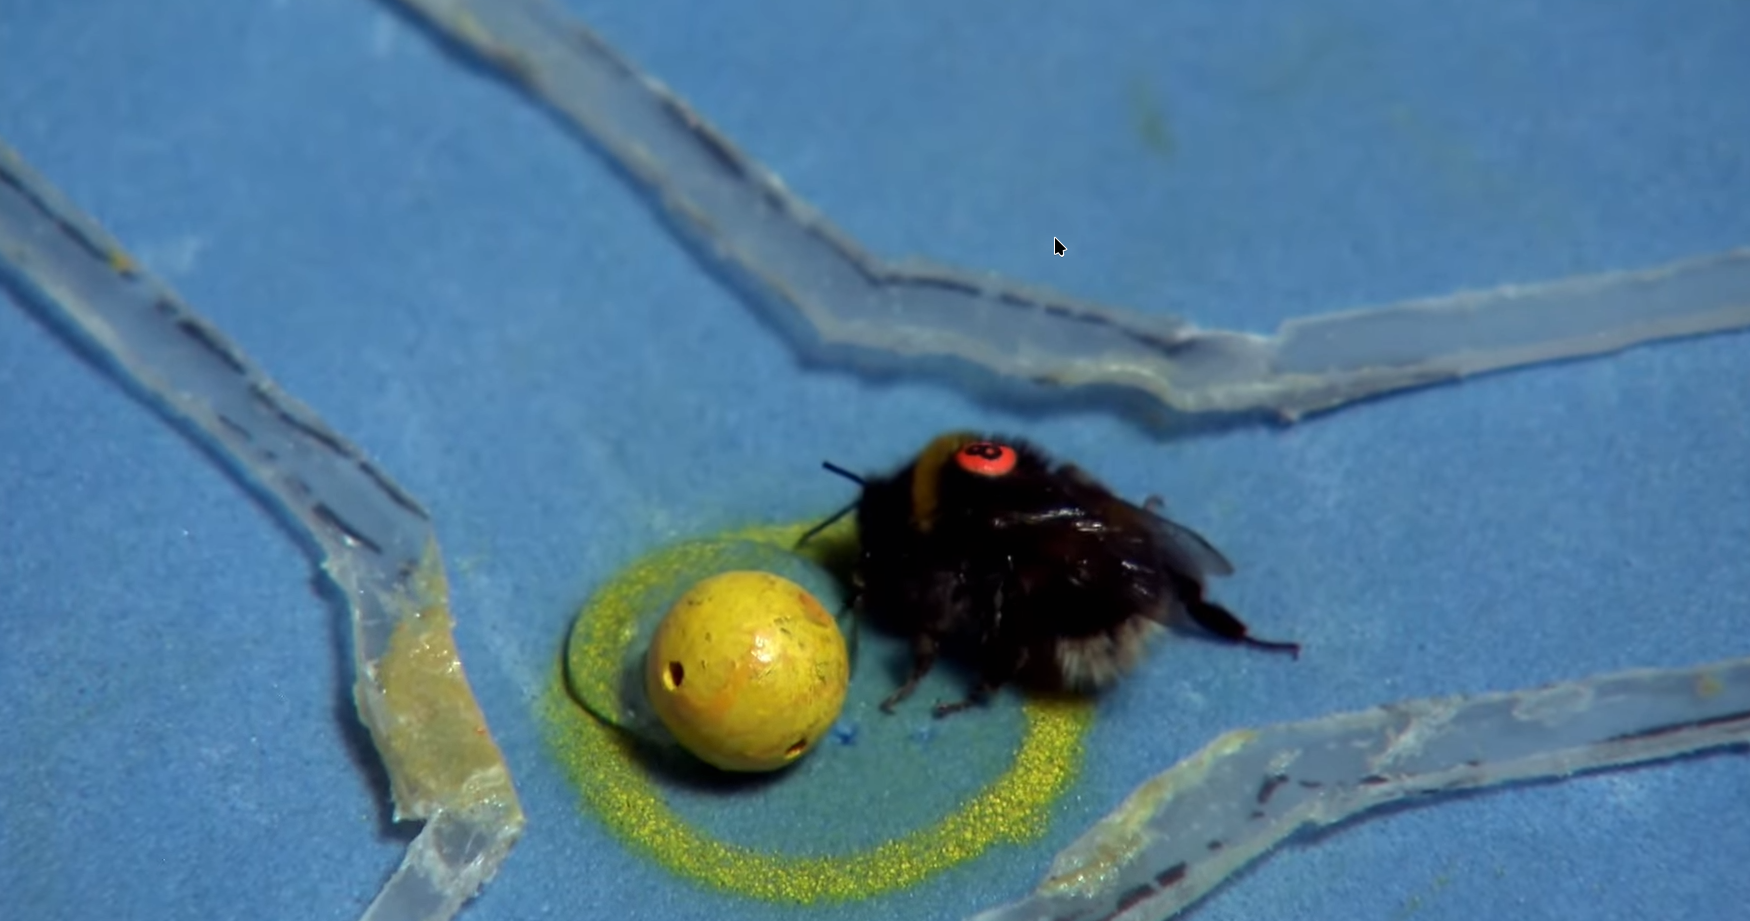
\includegraphics[width=2.93519in,height=1.54964in]{figures/image15.png}}\href{https://www.youtube.com/watch?v=3eUGj21c22w}{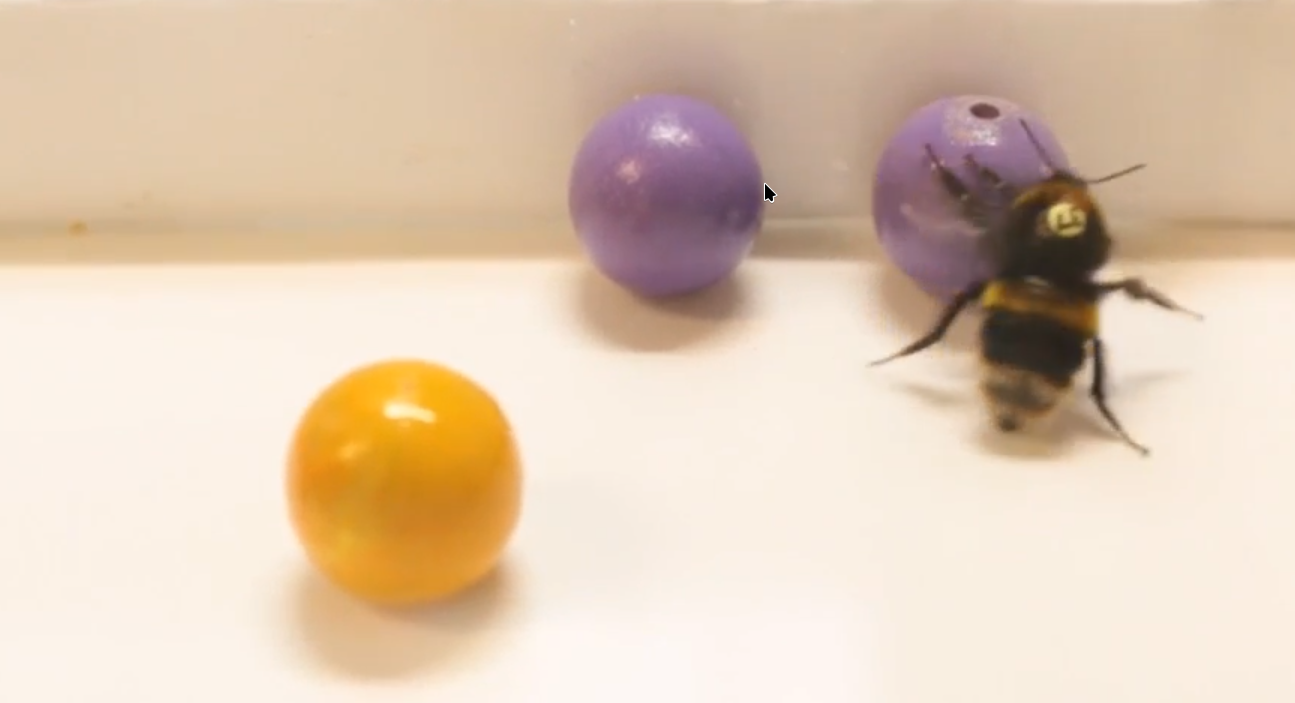
\includegraphics[width=2.27295in,height=1.23445in]{figures/image13.png}}\href{https://www.anura.it/works/hunters-hunter-portia-jumping-spider/}{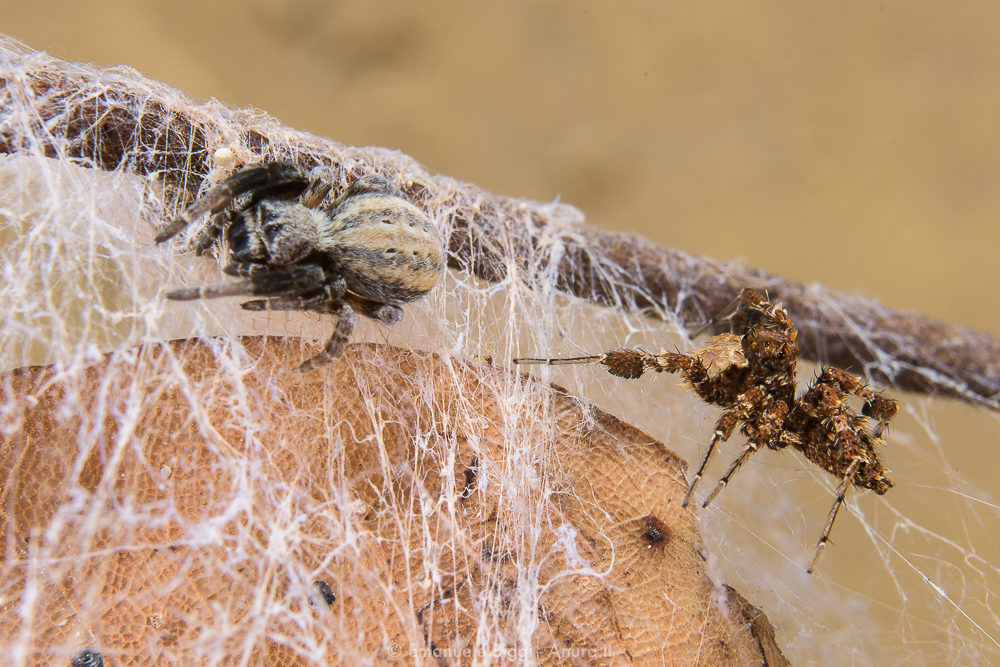
\includegraphics[width=2.26563in,height=1.50415in]{figures/image10.png}}

\href{https://www.britishecologicalsociety.org/ants-adapt-tool-use-to-avoid-drowning/}{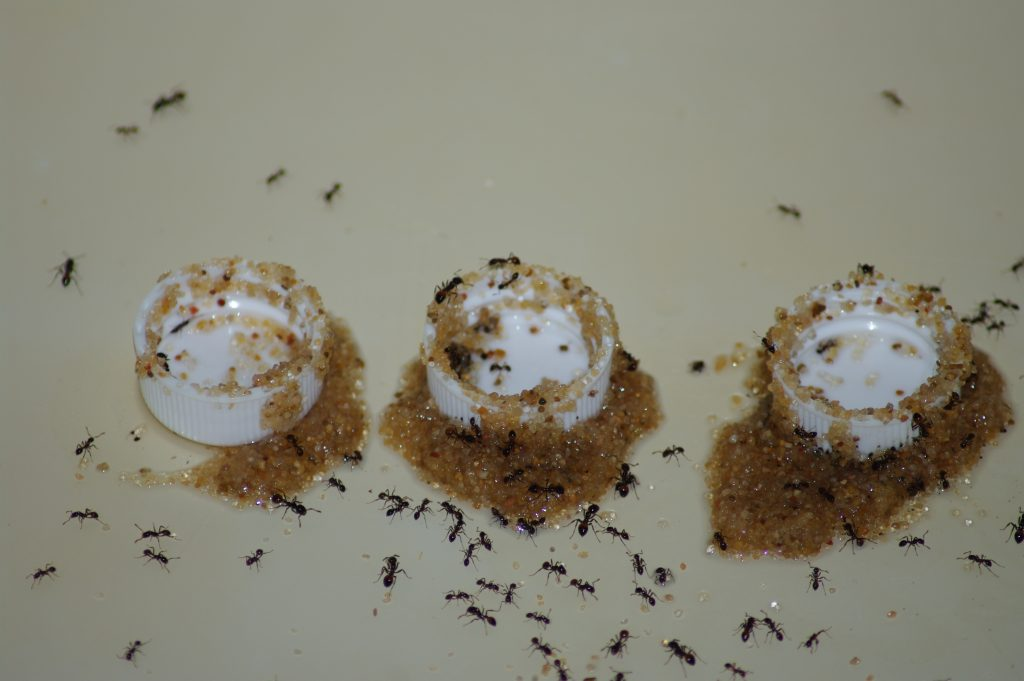
\includegraphics[width=3.99086in,height=2.65407in]{figures/image5.png}}

\begin{enumerate}
\def\labelenumi{\arabic{enumi}.}
\item
  Biological organisms are adaptive on different levels of organization
\item
  Learn without backpropagation
\item
  All cells types can communicate with each other
\item
  Demonstrate goal-directed behaviour
\end{enumerate}

Current neural architectures are more fragile than biological ones.

Our motivation is to determine if current intrinsic motivation methods would lead to learning and behaviour types observable in insects. Whether these types of behaviours are reproducible with intrinsic rewards.

Does intrinsic motivation in RL lead level 2 and level 3 learning types:

\begin{enumerate}
\def\labelenumi{\arabic{enumi})}
\item
  Does it lead to emergent communication and cooperation?
\item
  Lead to observational learning?
\item
  Does it lead to play and episodic learning?
\end{enumerate}

\section{Basic math definitions}\label{basic-math-definitions}

Mutual information of two random variables Y, Z

\(I(Y;\ Z)\ : = \ D_{KL}(P(Y,\ Z)\ ||\ P(Y)P(Z))\) (1)

Kullback-Liebner divergence

\(D_{KL}(P\ ||\ Q)\  = \ \sum_{x}^{}P(x)\ log\ \frac{P(x)}{Q(x)}\  = \ E_{P}\lbrack log\ P(x)\  - \ log\ Q(x)\rbrack\) (2)

Here P, Q - probability distribution over the same sample space.

Mutual information

\(I(Y;Z)\ : = \ H(Y)\  - \ H(Y\ |\ Z)\  = \ H(Z)\  - \ H(Z|Y)\ \) (3)

Here H is entropy.

H(Y) = - \(\sum_{y}^{}p(y)\ log\ p(y)\)

Pointwise mutual information \(PMI(x,y) = log\ \frac{P(x,y)}{P(x) \cdot P(y)}\) where x, and y are events, not random variables.

\(I(X;Y)\  = \ {\mathbb{E}}_{(x,y) \sim p(x,y)}\ \lbrack\ PMI(x,y)\ \rbrack\)

Reinforcement learning objective - maximising expected discounted reward

\(J(\pi)\ : = \ E_{\pi}\ \lbrack\ \sum_{t}\ \gamma ᵗ\ r(s_{t})\ \rbrack\) \hl{(6)}

\(\pi\) \hl{- policy.} \(\gamma\) \hl{- discount factor in range (0, 1)} \(s_{t}\) \hl{- state at time t.}

\section{Empowerment in reinforcement learning}\label{empowerment-in-reinforcement-learning}

Mutual information between agent's action and observable states can be used as reward. Empowerment is defined as conditional mutual information between action taken in the current state, and the next state \(I(A;S' \mid s)\)

\(I(A;S' \mid s) = D_{KL}(p(a,s' \mid s) \parallel p(a \mid s)p(s' \mid s))\) (4)

\(I(A;S' \mid s) = H(S' \mid s) - H(S' \mid A,s)\) (5)

I(A ; S' \textbar{} s) = H(A \textbar{} s) − H(A \textbar{} S',s)

First expand \(H(S' \mid s)\):

\(H(S' \mid s) = \  - \ \sum_{s'}\ p(s' \mid s)\ log\ p(s' \mid s)\)

\(p(s' \mid s) = \sum_{a}\  p(a,s' \mid s)\) then \(H(S' \mid s)\  = - \ \sum_{s',a}\  p(a,s' \mid s)\ log\ p(s' \mid s)\  = \  - E_{p(a,s' \mid s)\ }\ log\ p(s' \mid s)\ \)

Second term \(H(S' \mid A,s)\)

\(H(S' \mid A,s) = \  - \sum_{a,s'}\  p(a,s' \mid s)\ log\ p(s' \mid a,s)\  = - E_{p(a,s' \mid s)\ }\ log\ p(s' \mid a,s)\ \)

Substitute back in 5:

\(I(A;S' \mid s) =\) \(- E_{p(a,s' \mid s)\ }\ log\ p(s' \mid s)\)

\(I(A;S' \mid s) = E_{p(a,s' \mid s)}\lbrack log\ p(s' \mid a,s) - log\ p(s' \mid s)\rbrack\)

Here s is current state, \(S'\) is the next state and \(A\) is action taken in state s.

\(A\) and \(S'\) are random variables but \(s\) is not.

It's important to note that removing conditioning on the current state \(s\), as in \(I(A;S'\)) or I(A; S) will lead to a degenerate solution.

Maximising H(S') - H(S'\textbar A) means that future state S' should be predictable from action alone, and I(A; S) = H(S) - H(S\textbar A) means the agent should directly map the action to state.

What is the behavior that is encouraged by this type of reward?

First term that is maximised \(H(S' \mid s)\) is conditional entropy of future state \(S'\).

Entropy is low for spiky, concentrated probability distributions and high for more even distributions.

For example, entropy of a binary random variable \(p(s_{i})\  = \ 0.5\) will be 1 bit, with 10 possible outcomes with probability \(p(s_{i})\  = \ 0.1\) entropy is \textasciitilde3.32 bit.

So \(H(S' \mid s)\) is high then our agent visits a large and diverse set of states.

Second term is minimised: \(H(S' \mid A,s)\), this is the entropy of the future state given the current state and action. This term encourages policy to take actions that have predictable outcomes. For deterministic environment we have \(H(S' \mid A,s)\) = 0, so only the first term is optimised.

Consider this grid world, with actions up, down, left, right:

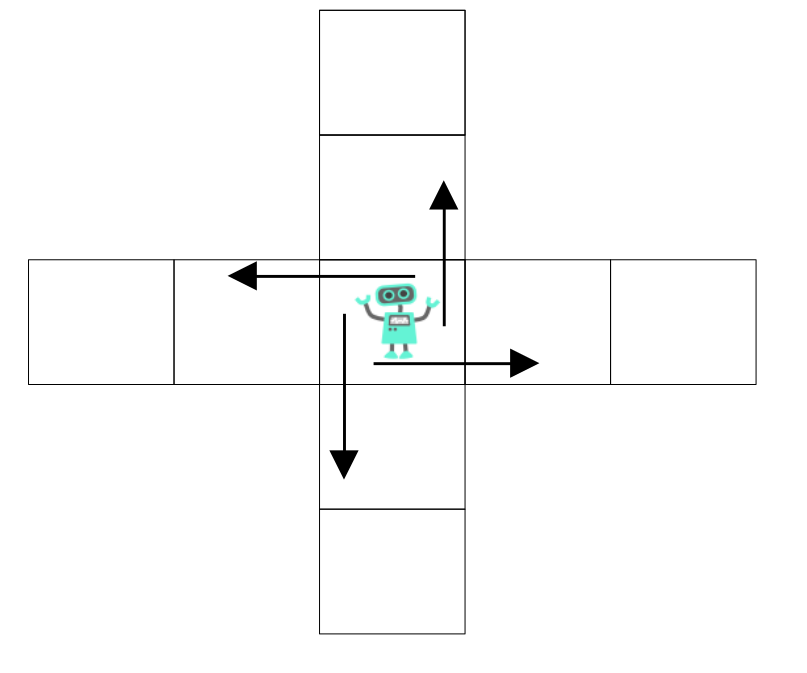
\includegraphics[width=5.27991in,height=4.40319in]{figures/image12.png}

Being in the central cell will have highest value of \(H(S' \mid s)\), \(- \sum_{i = 0}^{3}0.25\ log_{2}0.25\  = \ 2\) bit.

When we use empowerment in RL we maximise discounted accumulated empowerment over a trajectory: \(\sum_{t}^{}\gamma^{t}\ I(s_{t + 1},\ a|\ s_{t})\), follows from equation 6.

Here I is pointwise mutual information, MI is an expected value of PMI:

\(I(X;Y) = E_{X,Y}\lbrack PMI(X,Y)\rbrack = \ \sum_{x \in X}\sum_{y \in Y}\ \  P(x,y)\)

\subsection{Inverse model trick}\label{inverse-model-trick}

We can train a model that predicts action that leads from starting state s0 to end state s1. Here is how it works:

We can then estimate empowerment with

I(A ; S' \textbar{} s) = H(A \textbar{} s) − H(A \textbar{} S',s)

By definition we have for entropies:

H(A\textbar s) = - E {[} log p(a\textbar s) {]}

H(A \textbar{} S',s) = −E{[} log p(a\textbar S',s) {]}

p(a\textbar s) is known. It is distribution of actions under current policy \(\pi(a|s)\)

Distribution of actions given previous and future states p(a\textbar s',s) is not known, but we can introduce additional distribution q(a\textbar s',s) as follows:

\(H(A \mid S',s) = \  - \ E_{p(a,s' \mid s)}\ log\ \frac{p(a \mid S',s)\ q(a \mid S',s)}{q(a \mid S',s)}\ \)

Splitting the logarithm gives

\(H(A \mid S',s) = - E_{p(a,s' \mid s)}\ log\ q(a \mid S',s)\  - \ E_{p(a,s' \mid s)} log\ \frac{p(a \mid S',s)}{\ q(a \mid S',s)}\ \)

The second term is, by definition, the KL divergence. So:

\(H(A \mid S',s) = - E_{p(a,s' \mid s)}\ log\ q(a \mid S',s)\  - \ D_{KL}\lbrack\ \) \(p(a \mid S',s)||q(a \mid S',s)\) {]}

Now substituting this results back into empowerment equation gives:\\
\strut \\
\(I(A\ ;\ S'\ |\ s)\ \  = \  - \ E_{p(a|s)}\ \ log\ p(a|s)\  - (\  - \ E_{p(a,s' \mid s)}\ log\ q(a \mid S',s)\ \) \(- \ D_{KL}\lbrack\ p(a \mid S',s)||q(a \mid S',s)\rbrack\ )\)

\(I(A\ ;\ S'\ |\ s)\ \  = \ {E_{p(a,s' \mid s)}}_{}log\ q(a \mid S',s)\ \  - \ E_{p(a \mid s)}log\ p(a|s)\ \ \)\(\ \  + \ \ D_{KL}\lbrack\ p(a \mid S',s)||q(a \mid S',s)\rbrack\ \)

This gives us variation lower bound (ELBO) on empowerment, very similar to ELBO objective in variation autoencoder.

\(I(A\ ;\ S'\ |\ s)\ \  \geq {E_{p(a,s' \mid s)}}_{}log\ q(a \mid S',s)\ \  - \ E_{p(a \mid s)}log\ p(a|s)\ \ \)

We can minimise divergence \(D_{KL}\) term by maximising log-likelihood \(log\ q(a\ |\ s,\ s')\) on the on-policy samples (a, s, s'). Unlike mine/infonce we need only positive samples for this case.

For example if actions are continuous

\(q(a|s,\ s')\  = \mathcal{N}(a;\ \mu_{\theta}(s,\ s'),\ I)\ \)

We can obtain similar results for forward model that predicts future state from the equation

\(I(A;S' \mid s) = H(S' \mid s) - H(S' \mid A,s)\)

Though in this case we have to learn distribution of future state given current \(p(S'|s)\ \)which is usually a much harder problem than learning the inverse model.

For the most environments there are much less options for an action that have caused transition between states (s,s\textquotesingle) than for future states in p(s\textquotesingle\textbar s). For example in our grid world it's always only one possible action that causes transition between two cells, but there are 4 possible future states for the central cell.

The difficulty comes from simple models such as \(q(a|s,\ s')\  = \mathcal{N}(s';\ \mu_{\theta}(s),\ I)\ \)being inherently unimodal, not suitable for modeling a multimodal distribution. It's possible to make \(\mu_{\theta}(s)\) output parameter for e.g. mixture of several Gaussians, or use more advanced and difficult techniques.

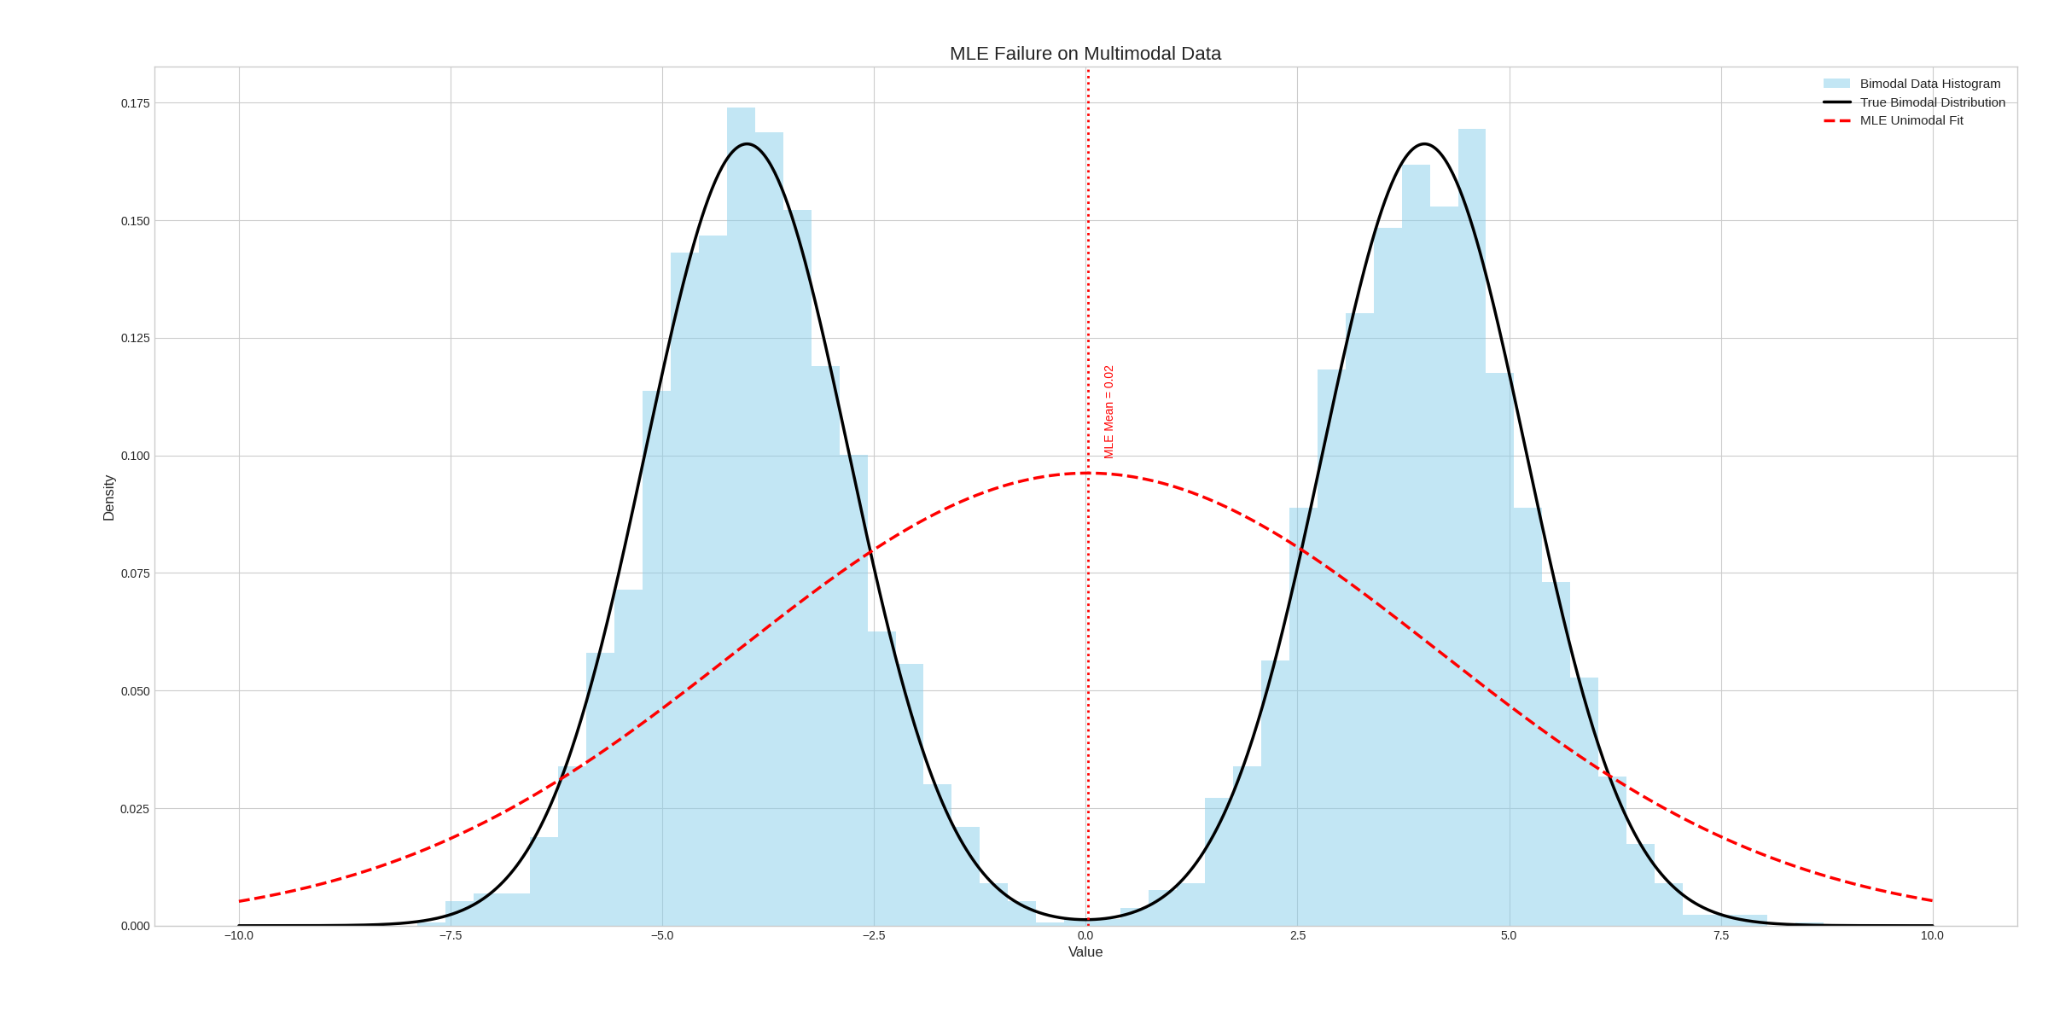
\includegraphics[width=21.33333in,height=10.60417in]{figures/image4.png}

Figure 1: MLE failure with single Normal distribution

Unimodal predictor will always output average and diffused(high variance) estimation for future state S.

\subsection{Continuous(differential) entropy}\label{continuousdifferential-entropy}

Continuous entropy behaves quite differently from discrete, in fact for a variable X with Delta-function density we have \(h_{X} = - \infty\).

If in inverse model reconstruction becomes possible to arbitrary precision, for example in deterministic environment empowerment may become infinite:

\(I(A;S' \mid s) = h(A \mid s) - h(A \mid S',s) = h(A \mid s) - ( - \infty) = \infty\)

Also for continuous actions it's possible to maximise empowerment by increasing actions magnitude. For normal distribution

\(h(A) = \frac{1}{2}\  log_{2}(2\pi\ e\ \sigma^{2})\) so policy will learn to maximise \(h(A \mid s)\) by increasing action range.

Natural solution is to constraint the range to \(A\  \in \lbrack a_{\min},\ a_{\max}\rbrack\) or restrict covariance.

To prevent entropy explosion in p(a∣s',s) we could add noise to observations:

\(p(a \mid s'\  + \ \epsilon,s)\ \)cannot perfectly recover \(a\) anymore keeping entropy and empowerment finite. For more detailed treatment of continuous entropy and mutual information see ``Handbook of differential entropy'' 978-1-4665-8317-7.

\section{Multistep and single-step empowerment}\label{multistep-and-single-step-empowerment}

Consider this simple 2 step environment, it does xor on two actions, always returns 0 at t=0 and t=1 :

T = 0 T = 1 T = 2, return xor(actions)

observe 0→a0 →observe 0 → a1 → observe 1

observe 0→a0 →observe 0 → a0 → observe 0

observe 0→a1 →observe 0 → a0 → observe 1

observe 0→a1 →observe 0 → a1 → observe 0

\(O_{2}\) is independent from \(O_{1}\) and \(A_{1}\) and \(\ I(A_{1};S_{2}|\ s_{1})\  = \ 0\)

But \(\ I(A_{1}A_{2};S_{2}|\ s_{1})\  > \ 0\)

This would be two-step empowerment. We can define k-step empowerment as:

\(I_{k}(s0)\  \triangleq \ I(A_{0:k - 1}\ ;\ Sk\ │\ s0)\ \)

With intermediate states added it is called trajectory empowerment.

\(I_{k}(s_{0})\  \triangleq \ I(A_{0:k - 1}\ S_{1:\ k - 1};\ S_{k}\ │\ s_{0})\)

\subsubsection{Local Optima}\label{local-optima}

Many people enjoy computer games, they can even hook some humans into addictive patterns. Empowerment fits best among intrinsic motivations for modelling this effect. The reward is high where there are many visited states, but the environment is controllable. An agent might get obsessed with flipping a switch that has tons of settings because it's easy to manipulate and offers immediate, predictable feedback. In the real world there are resource constraints which won't allow us to fixate on a game. Prediction-error driven agents can get stuck observing a noise source. Similarly, empowerment-driven agent can stuck observing controllable objects with many states.

There are many possible workarounds. People like playing video games, but even ones with addiction won't stick there because of resource constraints. Any real environment has resource constraints and resource sources so we can introduce resource constraints into virtual environments.

Lets add to the state energy coordinate \hl{\emph{e}∈{[}0,1{]}}

\(S\  = \ (s,\ e)\)

Every action consumes Δe \textgreater{} 0

When \(e < e_{crit}\) the motor controller becomes noisy or certain

actions are disabled. Formally, p(s'∣s,a) grows broader ⇒ H(S'∣a,s) increases, thus lowering empowerment. There are recharge states \(s_{charge}\)

(pick-ups, charging pads, food) that reset \emph{e} upward.

Therefore a pure empowerment maximiser already obtains an intrinsic

drive to:

 1. stay away from low-energy states,\\
 2. periodically reach recharge regions,\\
 3. optimise its action sequence for long-term discounted reward.

I.e. the agent behaves like a living organism: forage → play/act →

return to base → repeat.

It is easy to introduce to environment with direct biological analogy, like predator-pray, and harder for other cases. On the other hand in a multi-agent world it might not be necessary. Other agents will natural brake against ``camping on a toy'' behaviour.

• Disturbance: other agents policy injects variability into transition probability \(p(s_{t + 1}|\ a_{t},\ s_{t})\) leading to increase of entropy of future state \(H(S' \mid A,s)\) conditional on action.

• resource competition: agent must keep discovering new high-control niches or defend the old one.

\hl{• Non-stationary dynamics: camping behaviour might become impossible as time goes due to the non-stationary environment itself.}

When the multi-agent cure might fail:

1. Predictable opponents\\
If other agents adopt highly regular or submissive policies,

H(S'∣A,s) can still be low → empowerment can stay high.

2. Collusion / territorial partition\\
Agents may implicitly agree on ``you keep toy \#1, I keep toy \#2''. Each finds a private controllable niche.

\section{Empowerment in communication}\label{empowerment-in-communication}

Now consider there are two agents a and b that can send messages to each other from some alphabet M.

High empowerment reward is achievable for both agents in such a situation.

Agent a selects message m randomly and sends it to b. If b responds predictably, e.g. (m + 1) \% \textbar A\textbar{} then

We have high\(\ P(S' \mid m,s0)\)\(\)and high H(S'\textbar s0) (since response can't be predicted without knowing the message). Since next state now is completely predictable we get empowerment equals to H(A\textbar s). In this case both agents will achieve maximum reward with uniform distribution over M.

Achievable empowerment is approximately log\textbar A\textbar{}

With limited bandwidth agents might develop some kind of turn-taking schedules. But with energy constraints agents might refuse sending a response, lowering other agent's empowerment.

\section{MINE and InfoNCE}\label{mine-and-infonce}

\subsection{Mutual information neural estimation is defined as this objective:}\label{mutual-information-neural-estimation-is-defined-as-this-objective}

\begin{itemize}
\item
  \({I(Y,X)\  = \ D}_{KL}(P\ ||\ Q)\  > = \ sup_{T:\Omega \rightarrow R}\ E_{P}\ P\lbrack T(Y,X)\rbrack\  - \ log\ E_{Q}\lbrack e^{T(Y,X)}\rbrack\)
\end{itemize}

Where P(Y, Z) is joint distribution and Q = P(Y)P(Z) is marginal distributions.

T is a function returning real number \(T(Y,\ Z)\  \rightarrow \ R\). We approximate T by neural network \(T_{\theta}\)(Y, Z) and use gradient ascend to find supremum.

At training time we just need Monte-Carlo samples for both terms.

Loss is \(\sum_{}^{}\frac{1}{N_{b}}T_{\theta}(x,\ y)\  - \sum_{}^{}\frac{1}{N_{b}}T_{\theta}(\widehat{x},\ \widehat{y})\ \)

\(\widehat{x}\), \(\ \widehat{y}\) - samples from marginal distributions, to obtain them we can draw separate batches for x and y or just shuffle x or y from the same batch that is used in \(T_{\theta}(x,\ y)\).

It can be proofed that supremum achieved when \(T*(X,\ Y)\  = \ log\ \frac{P_{X,Y}}{Q_{X,Y}}\  + \ C\ \)

\(log\ \frac{P_{X,Y}\ }{Q_{X,Y}} = \ log\ P\  - \ log\ Q\  = log\ p(X,\ Y)\  - \ log\ p(X)P(Y)\ \) is just pointwise mutual information.

For empowerment estimation we have two random variables A and S, but this is conditioned on current stats s.

Plugging A and S in T gives

T(A;S'\textbar s) = log P(A;S'\textbar s) - log (P(A\textbar s) P(S'\textbar s) + c

T(A;S'\textbar s) = log( \hl{p(S\textquotesingle\textbar A,s)p(A\textbar s)) -} log (P(A\textbar s) P(S'\textbar s) + c

\(T(A;S’|s)\  = \ log\ p(S'|A,s)\  + \ log\ p(A|s)\  - \ log\ p(A|s)\  - \ log\ p(S’|s)\  + \ c\)

\(T(A;S’|s)\  = \ log\ p(S'|A,s)\  - \ log\ p(S’|s)\  + \ c\)

\(I(A;S' \mid s) = H(S' \mid s) - H(S' \mid A,s)\  = - \ E\ \lbrack\ log\ P(S' \mid s)\rbrack\  - \ ( - \ E\ \lbrack log\ p(S’|A,\ s)\rbrack\))

\(I_{A,S'\ \sim\pi}(A;S' \mid s)\  = \ E\lbrack\ log\ p(S’|A,\ s)\  - \ log\ P(S' \mid s)\ \rbrack\)

Thus trained T-function directly gives a point estimate of empowerment.

The catch is we can't anymore sample negatives that easily. Shuffling batch will give us \(I(S';(S,\ A))\) because shuffling will approximate S' \textasciitilde{} p(S') - unconditional distribution instead of \(P(S' \mid s)\).

\(I((S,A);S') = E_{S \sim p(s)}E_{A \sim \pi( \cdot \mid S)}E_{S' \sim p( \cdot \mid S,A)} log\frac{\ p(S' \mid S,A)}{p(S')}\)

\(I(S';A|s) = E_{A \sim \pi( \cdot \mid S)}E_{S' \sim p( \cdot \mid S,A)} log\frac{\ p(S' \mid S = s,A)}{p(S'|S = s)}\)

With \(I((S,A);S’) = I(S;S’) + I(A;S’ \mid S)\) \hl{\hfill\break
}

Compare \(I(S;S’)\) \hl{}to \(I(A;S' \mid s)\):

\(I(S;S’)\  = \ H(S’)\  - \ H(S'|S)\)

\(I(A;S' \mid s) = H(S' \mid s) - H(S' \mid A,s)\)

So we have conflicting term H(S'\textbar S) that cancels out.

\(I((S,A);S’)\) \emph{\hl{=}} \(H(S’)\ \)\(- H(S' \mid A,s)\)

\section{WORLD MODELS}\label{world-models}

World models are models that infer world state from observations and predict how this state evolves given actions. This allows to train policy in virtual episodes.

Here we describe prominent models Dreamer v3 and TWISTER and their components.

\href{https://arxiv.org/pdf/1807.03748}{\ul{https://arxiv.org/pdf/1807.03748}}

\href{https://arxiv.org/pdf/2301.04104}{\ul{https://arxiv.org/pdf/2301.04104}}

\href{https://arxiv.org/pdf/2503.04416}{\ul{https://arxiv.org/pdf/2503.04416}}

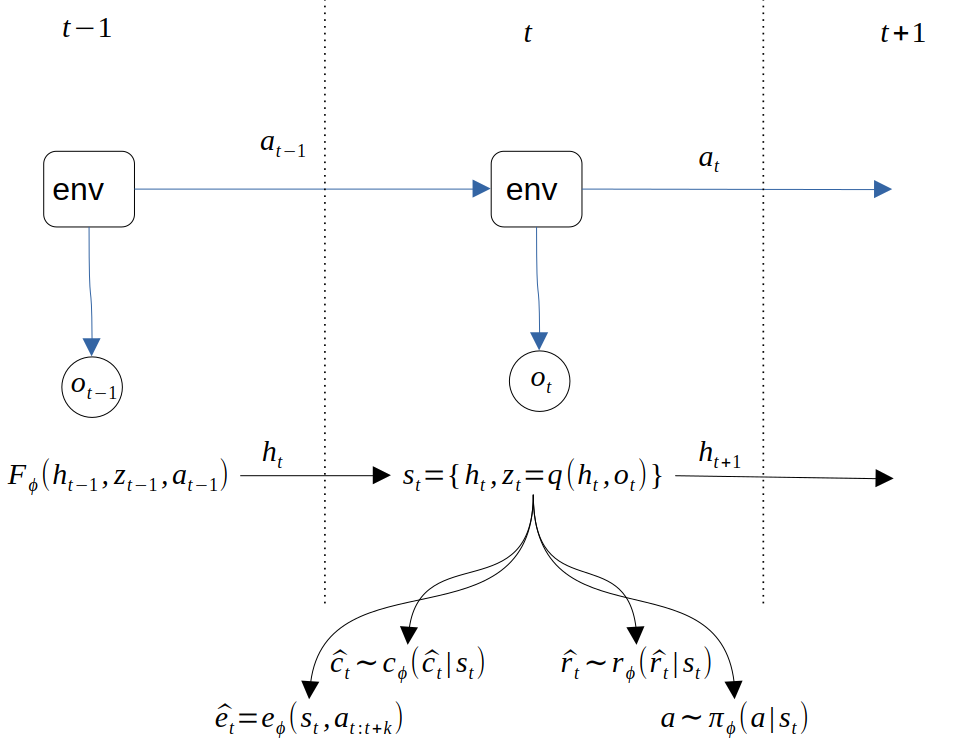
\includegraphics[width=9.92708in,height=7.73958in]{figures/image6.png}

Key components of DREAMER/TWISTER

\begin{quote}
\(h_{t}\  = F\phi(h_{t - 1},z_{t - 1},a_{t - 1})\) - context encoder e.g. RNN or transformer.

\({\widehat{z}}_{t}\  \sim \ d_{\phi}({\widehat{z}}_{t}\ |\ h_{t})\) - dynamics predictor: models distribution of world state given context. Virtually this predicts how world changes given previous state and action \(a_{t - 1}\)which encoded in \(h_{t}\)

\(z_{t}\  \sim \ q_{\phi}(z_{t}\ |\ o_{t},...)\) - observation encoder, models distribution of \(z_{t}\) given current observation \(o_{t}\) e.g. VAE encoder. In dreamer v3 its \(z_{t}\  \sim \ q_{\phi}(*\ |\ o_{t},\ h_{t})\) .

\(s_{t}\  = \ \{ h_{t},\ z_{t}\}\) - concatenation of context and world state.

\({\widehat{o}}_{t}\  \sim \ p_{\phi}({\widehat{o}}_{t}\ |\ z_{t})\) - observation decoder, models distribution for observations e.g. VAE decoder, in dreamer it's \({\widehat{o}}_{t}\  \sim \ p_{\phi}({\widehat{o}}_{t}\ |\ s_{t})\).
\end{quote}

\({\widehat{e}}_{t} = \ u\ (z_{t})\)\(\)- model that projects world states to embedding space.

\begin{quote}
\({\widehat{e}}_{t:t + k}\  = \ w_{\phi}\ (s_{t},\ a_{t:t + k})\) - predicted embeddings given state and actions
\end{quote}

\({\widehat{r}}_{t}\  \sim \ r_{\phi}({\widehat{r}}_{t}\ |\ s_{t})\) - predicted reward for current transition

\({\widehat{c}}_{t}\  \sim \ c_{\phi}({\widehat{c}}_{t}\ |\ s_{t})\) - predicted episode continuation/termination

losses:

\begin{quote}
\({\widehat{z}}_{t}{\sim d}_{\phi}\) is learnt with KL divergence with \(z_{t}\) produced by observation encoder.

\(q_{\phi}\) and \(p_{\phi}\) are trained with whatever encoder-decoder loss is suitable e.g. ELBO loss.

\(w_{\phi}\) is trained with constructive loss with projection \(u(\)\(z_{t}\)) of observed \(z_{t}\) to predicted \({\widehat{e}}_{t:t + k}\)

It is also possible to learn other useful signals such as rewards and episode termination.
\end{quote}

\subsection{Action Conditioned (AC-CPC)}\label{action-conditioned-ac-cpc}

This is TWISTER component that is responsible for \({\widehat{e}}_{t} = \ u\ (z_{t})\)\(\)training.

This is an architecture that allows compressing high-dimensional observations into useful representations.

RSSM stands for Recurrent State-Space Model. This is a part of dreamer that constitutes the world model. In TWISTER it is TSSM - transformer instead of recurrent model.

There are two key differences:

\begin{enumerate}
\def\labelenumi{\arabic{enumi})}
\item
  \textbf{Dreamer} updates distribution \({\widehat{z}}_{t}\  \sim \ d_{\phi}(*\ |\ h_{t})\) to match different encoder: \(z_{t}\  \sim \ q_{\phi}(*\ |\ o_{t},\ h_{t})\).
\end{enumerate}

\begin{quote}
\hl{This is very similar to recursive Bayesian estimation or Bayesian filtering, very similar to the inference in the hidden-markov model. Unlike TWISTER which uses} \(z_{t}\  \sim \ q_{\phi}(*\ |\ o_{t})\)
\end{quote}

\begin{enumerate}
\def\labelenumi{\arabic{enumi})}
\setcounter{enumi}{1}
\item
  AC-CPC/TWISTER contrastive loss for embeddings additionally to reconstructive loss in Dreamer.
\end{enumerate}

Another minor difference decoder in dreamer is \({\widehat{o}}_{t}\  \sim \ p_{\phi}({\widehat{o}}_{t}\ |\ s_{t})\)

Having said that it helps to concatenate many observations \(o_{t}\) or use dreamer style encoder \(\ q_{\phi}(z_{t}\ |\ o_{t},\ h_{t})\) for AC-CPC\hl{.}

Both methods are reported to work best with discrete distribution of world states \(z_{t}\). though can be used with different distributions.

\hl{o0, a0, o1, a1, o2, a2, o3, a3...}

\hl{h0=0, z0 = qϕ(h0, o0), h1=Fϕ(z0, h0, a0), z1 = qϕ(h1, o1)...}

\hl{z0=0, hat z1 = dϕ(h1), hat z2 = dϕ(h2)}

\hl{}

\hl{s0 = {[} h0, z0{]}, s1 = {[}h1, z1{]}...}

\hl{prior hat z2 = dϕ(h2)}

\hl{s0 -\textgreater{} a0,}

\hl{s1 -\textgreater{} a1}

\hl{and for ac-cpc starting from h1:}

\hl{e10 = f(h1) - conditioned by a0 via h1}

\hl{e12 = f(h1, hat z1, a1)}

\hl{e13 = f(h1, hat z1, a1, a2)}

\hl{with positives e10 \textless-\textgreater{} z1, e12 \textless-\textgreater{} z2, e13 \textless-\textgreater{} z3\ldots{}}

\hl{Quantity that is being optimised is this loss:\\
}

\(L_{InfoNCE}\  = \  - \frac{1}{N}\ log\ \frac{e^{{s^{k}}_{ii}}}{e^{{s^{k}}_{ii}}\  + \ \sum_{j \neq i}^{}e^{{s^{k}}_{ij}}}\)

With s being similarity measure between embedding and latent variable z(z is being projected to the embedding space with a mlp). N is batch size.

Mutual information between matching embeddings e and latent states z is being simply:

\(I(e_{};\ z_{})\  > = \ log\ N\  - \ L_{InfoNCE}\)

In twister this is used only for descriptor training, but what if we use this MI estimation for reward? Is it similar to empowerment? If we assume that e and z are good enough representations of it's inputs we could write:\\
\strut \\
\(I(e_{};\ z_{})\  \approx \ I({(h}_{t},\ a_{t:t + k}),\ h_{t + k})\  \approx \ I({(s}_{t},\ A),\ S')\)

By chain rule for MI(see appendix)

\(I((s,\ A);\ S')\  = \ I(s\ ;\ S')\  + I(A;S' \mid s)\)

As you can see this quantity can reward behaviour when future trajectory is predictable even without knowing action.

Expand:

\(I(s\ ;\ S') = \ H(S')\  - \ H(S'|s)\)

\(I(A;S' \mid s)\  = \ H(S' \mid s) - H(S' \mid A,s)\ \) - multistep empowerment

\(H(S')\  - \ H(S'|s)\) + \(H(S' \mid s) - H(S' \mid A,s)\) = \(H(S') - H(S' \mid A,s)\)

\(I((s,\ A);\ S')\) = \(H(S') - H(S' \mid A,s)\)

This is difference \(H(S')\) vs \(H(S' \mid s)\) tells us what we are trying to distinguish/predict from s and A. AC-CPC uses for negatives all possible states S in a batch. While \(H(S' \mid s)\) would require us to construct negatives only from states we could arrive from the current state \(s\)!

\section{Diversity is all you need}\label{diversity-is-all-you-need}

The goal of this method is to make an agent learn different skills in an unsupervised manner.

In this method we pass to the policy additional parameter z that is sampled from a random distribution(categorical or normal). Z ∼ p(z). Policy conditioned on z is called skill. Training objective has tree parts:

1) Mutual information between states and skills I(S;Z) is maximised

2) MI between actions and skills given the state is minimised I(A;Z \textbar{} S)

3) Entropy of actions given state is maximised H{[}A \textbar{} S{]}

\(max\ F(\theta)\  \triangleq \ I(S;Z)\  + \ H\lbrack A\ |\ S\rbrack\  - \ I(A;Z\ |\ S)\) (1)

\(\ \ \ \  = \ (H\lbrack Z\rbrack\  - \ H\lbrack Z\ |\ S\rbrack)\  + \ H\lbrack A\ |\ S\rbrack\  - \ (H\lbrack A\ |\ S\rbrack\  - \ H\lbrack A\ |\ S,\ Z\rbrack)\)

\(= \ H\lbrack Z\rbrack\  - \ H\lbrack Z\ |\ S\rbrack\  + \ H\lbrack A\ |\ S,\ Z\rbrack\) (2)

\(H\lbrack Z\rbrack\) is entropy of skill distribution - constant.

Conditional entropy of skill distribution can be rewritten as:

\(H\lbrack Z\ |\ S\rbrack\  = H(S,\ Z)\  - \ H(S)\)

\(H\lbrack Z\ |\ S\rbrack\ \)= H{[}S\textbar Z{]} - H(Z)

This will help us to understand when exactly the reward will be high and when low.

Substituting it into original equation:\\
\(F(\theta)\  = \ \ H\lbrack Z\rbrack\) - (\(H(S,\ Z)\  - \ H(S)\) ) + \(H\lbrack A\ |\ S,\ Z\rbrack\)

= \(\ H\lbrack Z\rbrack\ \)- \(H(S,\ Z)\) + \(H(S)\) + \(H\lbrack A\ |\ S,\ Z\rbrack\)

\hl{Expand joint entropy of skills and states:}

\hl{H(S, Z) = H(S\textbar Z) + H(Z) = H(Z\textbar S) + H(S)}

\(F(\theta)\  =\) \(H\lbrack Z\rbrack\) - ( \hl{H(S\textbar Z) + H(Z) ) + H(S) +} \(H\lbrack A\ |\ S,\ Z\rbrack\)

= \(H\lbrack Z\rbrack\) - \hl{H(S\textbar Z)- H(Z) + H(S) +} \(H\lbrack A\ |\ S,\ Z\rbrack\)

= \hl{H(S) +} \(H\lbrack A\ |\ S,\ Z\rbrack\) - \hl{H(S\textbar Z)}

\hl{This form helps to understand what behaviour is encouraged by this reward.}

\hl{First term \textbf{H(S)} maximises entropy of states = encourages policy to visit many states.}

\(H\lbrack A\ |\ S,\ Z\rbrack\) - conditional entropy of action given state and skill - encourages policy to apply different actions given skill and state. Equivalently this means it should be hard to guess skill from action alone.

Also maximising this term makes it so knowing state + action doesn't give more information about skill than knowing just state alone.

H(S\textbar Z) is minimised. If it is low we have a small number of states which are visited by given skill.\\
\strut \\
Using definition I(Z;A∣S)=H(A∣S)−H(A∣S,Z)

\emph{H}(\emph{A}∣\emph{S},\emph{Z}) = \emph{H}(\emph{A}∣\emph{S}) - \emph{I}(\emph{Z};\emph{A}∣\emph{S})

So, \(F(\theta) = \ H(S)\  + \ H(A \mid S)\  - \ H(S|Z)\  - \ I(Z;A \mid S)\ \) =

\(\ H(Z) + \ H(A \mid S) - \ H(Z\ |\ S)\  - \ I(Z;A \mid S)\)

Max H(S) = maximise the number of visited states.

Max H(A∣S) = maximise the number of actions taken in any particular state.

Min H(S\textbar Z) = minimise the number of states visited by a particular skill.

Min I(Z;A∣S) = all actions are more or less the same for all skills.

Min H(S\textbar Z) = skill can be used to predict S

\hl{\hfill\break
This objective can be implemented as:}

\(H(Z\ |\ S)\) = \(- \sum_{}^{}p(s,\ z)\ log\frac{p(s,\ z)}{p(s)} = \ E\lbrack - log\ p(z|s)\rbrack\)

\(H(Z)\) = \(- \sum_{}^{}p(\)z) log p(z) = E{[}-log p(z){]}

\(\ H(A \mid S,Z)\) = \(- \sum_{}^{}p(s,z)\sum_{}^{}p(a|s,\ z)\ log\ p(a|\ s,z)\  = \ E_{s,z}\lbrack - \sum_{}^{}p(a|s,\ z)log\ p(a|\ s,z)\ \rbrack\ \) = \(\ {- E}_{s,z,a}\lbrack log\ p(a|\ s,z)\ \rbrack\)

\(F(\theta)\  = \ E\lbrack - log\ p(z)\rbrack\  - \ E\lbrack - log\ p(z|s)\rbrack\  + \ E\lbrack - log\ p(a|\ s,z)\ \rbrack = \ E\lbrack\ \ log\ p(z|s)\  - log\ p(z)\ \  - log\ p(a|\ s,z)\ \ \ \ \ \ \ \ \ \ \rbrack\)

Probability of skill given state p(z\textbar s) is approximated by a neural network predictor \(\phi_{\theta}(s) - > z\ \)

log \(p(a|\ s,z)\) is just policy entropy log πθ(a\textbar{} s,z). It can be included in the reward or treated separately, like entropy reguliser as in soft actor-critic.

r(s, a\textbar{} z) = log φ(z \textbar{} s) − log p(z)

In principle it's possible to use forward density p(s\textbar z), but practically choice p(z\textbar s) is much easier to implement, since we don't know the ground truth distribution of S given skill.

Estimating φ(z∣s) is just a classification/regression problem; the target distribution over z is simple (uniform or Gaussian).

Estimating p(s∣z) is often a high-dimensional density problem (very hard for image observations).

Side by Side comparison with Empowerment

{\def\LTcaptype{none} % do not increment counter
\begin{longtable}[]{@{}
  >{\centering\arraybackslash}p{(\linewidth - 4\tabcolsep) * \real{0.2674}}
  >{\raggedright\arraybackslash}p{(\linewidth - 4\tabcolsep) * \real{0.3380}}
  >{\raggedright\arraybackslash}p{(\linewidth - 4\tabcolsep) * \real{0.3947}}@{}}
\toprule\noalign{}
\endhead
\bottomrule\noalign{}
\endlastfoot
& \textbf{Empowerment} & \textbf{DIAYN} \\
pushed up & \emph{p}(\emph{s`}∣\emph{a},\emph{s}) & \emph{p}(\emph{z}∣\emph{s}) \\
pushed down & \emph{p}(\emph{s'}∣\emph{s}) & \emph{p}(\emph{a}∣\emph{s},\emph{z}) \\
Encouraged property & Predictable consequences per action & States discriminate skills;

actions stay \emph{diverse} \\
Discouraged property & Small marginal next-state variability & Peaky action distribution inside a skill \\
\end{longtable}
}

In equation 1 variable Z is sampled ones per episode, S is picked uniformly from the whole trajectory, so the term \(\ H(Z\ |\ S\)) is computed with respect to the entire trajectory. But there are situations when examining multiple states might be desirable. We might be interested in achieving the same state by different means, for example robot can place a spoon in a mug either by taking a spoon and placing it or by trying to scoop the spoon. In this case intermediate states are clearly distinguish skill vector, but the end state is the same. By default DIAYN will try to avoid visiting the same state from two skills. We could counter it by either by adding external reward, curiosity, or adding structure to the skill vector.

\subsubsection{Structural DIAYN}\label{structural-diayn}

For example let vector z be concatenation of vectors \(z_{i}\).

If we choose to use just two vectors we will have:

\begin{itemize}
\item
  two latents z(1) and z(2) are concatenated \(z = \lbrack z^{(1)},\ z^{(2)}\rbrack\);
\end{itemize}

\begin{itemize}
\item
  the policy \(\pi(a \mid s,z^{(1)},\ z^{(2)})\) can use both parts all the time;
\item
  the discriminator at an early time slice tries to predict \(z^{(1)}\) only, ignoring \(z^{(2)}\);
\item
  the discriminator at the final state (or any late slice) predicts \(z^{(2)}\) only.
\end{itemize}

Any two skills that differ only in \(z^{(1)}\) therefore must converge to (almost) the same final state, reached via recognisably distinct trajectories.

We can also try to reconstruct all \(z^{(i\  < \ t)}\). In this case policy will be encouraged to treat early \(z^{i}\ \) as a high-level coarse plan or ``style'' and later \(z^{i}\) further nuancing the behavior. Other options such as using a sliding window are possible.

\section{Curiosity}\label{curiosity}

Curiosity reward can be a combination of a few things: surprise, for example in the form of prediction error, novelty and information gain.

Novelty is proportional to state visitation count: it is high for new states and low for frequently visited states.

Prediction error can be estimated from forward model:\(\ f(s,\ a)\  - > \ {\widehat{s}}_{t + 1}\)

Reward then is \(||s_{t + 1}\  - f(s,\ a)||_{}\ .\)

Information gain is a bit more complex. We have forward model \(f_{\theta}(s_{t + 1}|s,\ a)\) and distribution over its weights \(p(\theta|O_{t})\) given the history of transitions; \(\ O_{t}\  = \ \{(s_{\tau}\ ,\ a_{\tau}\ ,\ s'_{\tau})\}\) for \(\tau < t\).

Information gain is modeled as a change of distribution over parameters of forward model \(f_{\theta}(s_{t + 1}|s,\ a)\) given a new observation.

\(IG_{t} ≝ \ KL\ \lbrack\ p(\theta\ |\ O_{t}\  \cup \ O_{t + 1})\ \|\ p(\theta\ |\ O_{t})\ \rbrack\)

This can be approximated simply with improvement in prediction error.

That is \(r\  = ||\ f_{\theta_{k}}(s,\ a)\  - \ s_{t + 1}||_{}\ \  - ||_{}f_{\theta_{k + 1}}(s,\ a)\  - \ s_{t + 1}||_{}\)

Novelty and prediction error, unlike information gain are prone to noise-staring behaviour. That is, the reward is high when the agent observes pure noise. But there are easy workarounds. We can train a model that predicts action given previous and current states. \(g_{\theta}(s_{t + 1},\ s_{t})\  - > \ a\). Higher layers of this model can be used as feature extractors, that keep information only about controllable aspects of the environment. These features can be used then instead of raw states in novelty or surprise rewards.

Let's compare curiosity with empowerment.

Empowerment I(A;S'∣s)=H(S'∣s)−H(S'∣s,a)

Prediction error H(S'∣s,a)

State novelty H(S)

Given identity \(H(S') = I(S';\ S) + H(S' \mid S)\) we have H(S'∣s) is less or equal to \(H(S')\).

That is possible to have large \(H(S')\) and but small \(H(S' \mid S)\). Reverse is not true:

High \(H(S' \mid S)\) implies high \(H(S')\).

So maximising \(H(S')\) is not identical to maximizing \(H(S' \mid S)\). \(H(S' \mid S)\) encourages rewards states from which many different states can occur immediately(or in k-steps with k-steps empowerment). But H(S') rewards visiting the whole state space.

\section{}\label{section}

\section{Predictive Coding}\label{predictive-coding}

SFA

Invented by Laurenz Wiskott and Terrence Sejnowski (2002), Slow Feature Analysis is an unsupervised learning rule that extracts features whose values change as slowly as possible over time, although they are computed from an input stream that may itself vary quickly.

Let's say we have encoder neural network that transform each observation \(s_{t}\) in \(y_{t}\):

\(y_{t} = g(s_{t})\)

Slowness achieved with loss\\
\(L_{slowness} = \sum_{i = 1}^{}(y_{i} - y_{i - 1})2\)

In order to avoid degenerate solutions such as encoding each observation as zeros we require decorrelation, zero mean and unit variance for y.

Variance loss is defined as:

\(C_{Y} = \frac{1}{N} Y^{T}Y\) where Y is a concatenation of zero-centered vectors y.

\(L_{variance}\  = \ {\frac{1}{N}\sum_{i = 0}^{}C}_{Y}\lbrack i,i\rbrack\  - \ 1\)

And then correlation loss:

\(L_{correlation}\  = \ {\frac{1}{N}\| C}_{Y}\  \circ \ (1\ –\ I)\ \|_{F²}\) - Frobenius norm of the off-diagonal part.

Then objective is

\(L_{sfa}\  = \ L_{slowness}\  + \ L_{variance\ }\  + \ L_{correlation}\)

\section{Predictive information bonus and MDL}\label{predictive-information-bonus-and-mdl}

Imagine an agent that can see part of an image, can move on it and can change pixels. Empowerment alone won't produce interesting non-random looking images. We can use MI between patches of the image I(top-left, top-right) as reward in this case. This corresponds to regularized minimum description length. Regularization is needed to avoid obvious solutions when the image is blank. We can directly use any MI estimator or just use masked prediction \(p\theta(S_{mask}|S_{nonmasked})\). Trivial solutions will be avoided by standard entropy bonus for policy, by novelty bonus etc.

It\textquotesingle s also possible to use generative models such as VAE as approximator for description length.

\(description\ length\  \approx \  - \ log_{2}p\theta(s)\  < = \  - ELBO(s)\ /\ ln\ 2\ \)

\section{Problems with Empowerment and DIAYN}\label{problems-with-empowerment-and-diayn}

Single-step empowerment is short-sighted. It can even be zero for obviously easy environments as shown in the xor environment example. Multistep empowerment is better, but it can't be applied without modifications to high-frequency long-term environments like RTS games. On the other hand DIAYN objective is global in a sense that we can sample individual states from a trajectory for it's estimation, and it is the same expected value. But empowerment can't be zero given one-steps or two step estimation.

DIAYN\textquotesingle s objective is limited in a sense that it is just for learning skills. Humans or animals use skills to achieve certain goals, skills are combined and used in certain order. DIAYN objective says nothing about how skills should be combined. More in more realistic architecture an agent would pursue long-term goals switching between skills as the situation evolves.

Issues with empowerment can be addressed by introducing different time scales and state compression. In such case empowerment would be used to reward high-level actions that take many environmental steps to execute.

DIAYN skills can be such low-level actions. And skill selection can be trained by n-step empowerment.

If we choose to use empowerment for only high-level action selection we have to decide which states to use and which to omit. Consider RTS game with 640x480 video frames as observations. Suppose we have high-level actions pursue, build expand, build unit, attack, flee etc. We can't use just pixel observations at skill boundary. Both policy and empowerment estimator would require a feature vector that encodes strategic situations in the game + more detailed description of the current situation, that is exact unit position, recent events such as ``hero just died''.

Multi-layer SFA is a possible front-end to obtain the macro strategic state on which we measure empowerment or DIAYN MI.

{\def\LTcaptype{none} % do not increment counter
\begin{longtable}[]{@{}
  >{\raggedright\arraybackslash}p{(\linewidth - 0\tabcolsep) * \real{1.0000}}@{}}
\toprule\noalign{}
\endhead
\bottomrule\noalign{}
\endlastfoot
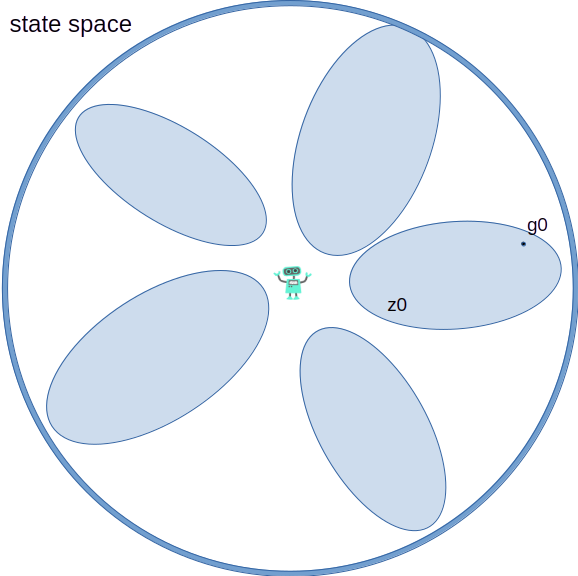
\includegraphics[width=6.02083in,height=6in]{figures/image9.png}

State space partition by DIAYN: no garanties that we can achieve a particular state g0. Increasing the number of skills will just make slices thinner. \\
\end{longtable}
}

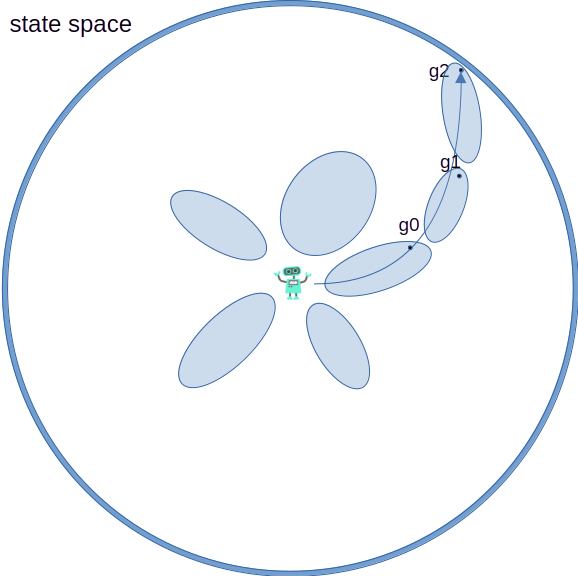
\includegraphics[width=6.02083in,height=6in]{figures/image1.png}

\subsection{}\label{section-1}

\subsection{}\label{section-2}

\subsection{}\label{section-3}

\section{\texorpdfstring{Math Appendix\\
}{Math Appendix }}\label{math-appendix}

\subsubsection{\texorpdfstring{Chain rule for Mutual information:\\
\strut \\
I(X, Y ; Z) = I(X ; Z) + I(Y ; Z \textbar{} X)}{Chain rule for Mutual information:  I(X, Y ; Z) = I(X ; Z) + I(Y ; Z \textbar{} X)}}\label{chain-rule-for-mutual-information-ix-y-z-ix-z-iy-z-x}

By definition we have\\
I(X, Y ; Z) = H(Z) - H(Z \textbar{} X, Y)

Expand I(X ; Z) and I(Y ; Z \textbar{} X) to entropies:

I(X ; Z) = H(Z) - H(Z \textbar{} X)

I(Y ; Z \textbar{} X) = H(Z \textbar{} X) - H(Z \textbar{} X, Y)

Compute sum:

I(X ; Z) + I(Y ; Z \textbar{} X) = H(Z) - H(Z \textbar{} X) + H(Z \textbar{} X) - H(Z \textbar{} X, Y) = H(Z) + H(Z \textbar{} X, Y)

\subsubsection{Donsker-Varadhan MI}\label{donsker-varadhan-mi}

We are starting from KL divergence \(D_{KL}(P\ ||\ Q)\  = \ \int_{}^{}p(x)\ log\ \frac{p(x)}{q(x)}dx\)

\textbf{Step 1. Define Gibbs density.}

Let T(x) be our arbitrary function. We create a new valid probability density, g(x), by weighting q(x) with \(e^{T(x)}\) to ensure g(x) integrates to 1, we must divide by a normalizing constant Z:

\begin{quote}
\(g(x)\  = \ \frac{e^{T(x)}q(x)\ }{Z}\)
\end{quote}

Where the constant Z is just the expected value over the distribution Q:

\begin{quote}
\(Z\  = \ \int_{\ }^{}e^{T(x)}q(x)\ dx\  = \ E_{Q}\ e^{T(x)}\)
\end{quote}

Step 2: Use the Non-Negativity of KL Divergence

\(D_{KL}(P\ ||\ Q)\  = \ \int_{}^{}p(x)\ log\ \frac{p(x)}{q(x)}dx \geq 0\)\\
\textbf{Step 3: Multiply by} \(\frac{q(x)\ }{q(x)}\)

\(log\ \frac{p(x)}{g(x)} = \ log\ \frac{p(x)}{q(x)}\ \frac{q(x)\ }{g(x)} = \ log\ \frac{p(x)}{q(x)}\  + \ log\ \frac{q(x)\ }{g(x)}\)

\(g(x)\  = \ \frac{e^{T(x)}q(x)\ }{Z}\  = > \ \frac{g(x)\ }{q(x)}\  = \frac{e^{T(x)}\ }{Z}\ \)

\(\frac{q(x)\ }{g(x)}\  = \frac{Z}{e^{T(x)}}\)

\(log\ \frac{q(x)\ }{g(x)}\  = log\ \frac{Z}{e^{T(x)}}\  = \ log\ Z\  - T(x)\ \)

\textbf{Step 4: Substitute and Solve}

\(\int_{}^{}p(x)\ log\ \frac{p(x)}{q(x)}\frac{q(x)\ }{g(x)}dx\  = \int_{}^{}(p(x)\ log\ \frac{p(x)}{q(x)}\  + \ log\ Z\  - \ T(x))\ dx\  \geq 0\ \)

First term\(\ \int_{}^{}(p(x)\ log\ \frac{p(x)}{q(x)}dx\) is \(D_{KL}(P\ ||\ Q)\ \)

Second term \(\int_{}^{}p(x)\ log\ Z\ dx\  = log\ Z\int_{}^{}p(x)\ dx\  = \ log\ Z\ *\ 1\  = \ log\ Z\ \ \)

Third term \(- \int_{}^{}p(x)T(x)\ dx\ \) is \(E_{P}T(x)\)

\(\ D_{KL}(P\ ||\ Q)\ \  + \ {log\ E}_{Q}\ e^{T(x)}\  - \ E_{P}\ T(x)\  \geq 0\)

\(D_{KL}(P\ ||\ Q) \geq E_{P}\ T(x)\  - log\ E_{Q}\ e^{T(x)}\ \ \)

We get mutual information with P being p(x, y) - joint density and Q being p(x)p(y) - the product of the marginal densities:

\(I(X;\ Y)\  \geq \ E_{P(X,Y)}T(x,y)\  - \ log\ E_{P(X)P(Y)}\ e^{T(x,y)}\)

\subsection{Value function}\label{value-function}

\section{Experiments, Options to try}\label{experiments-options-to-try}

Recurrent communicating cells trained with intrinsic motivation but without backpropagation.

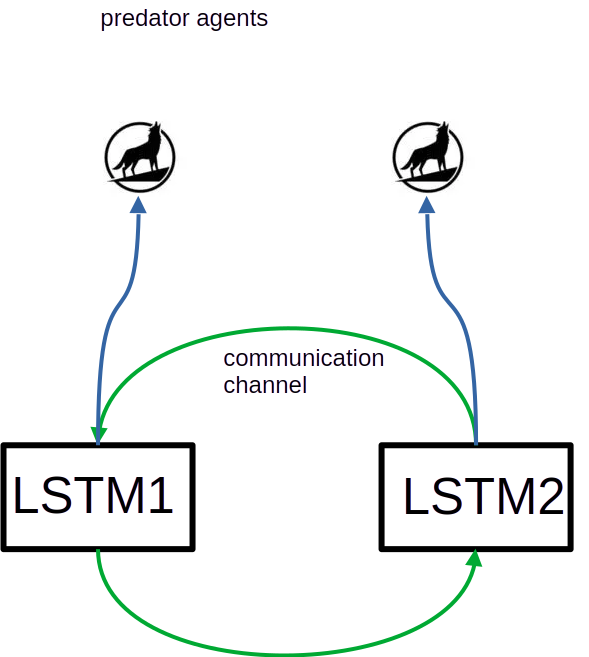
\includegraphics[width=3.55612in,height=3.96668in]{figures/image2.png}

Analogous to different types of cells having the same genome but different behaviour two LSTMs can share the same weights.

Predator-prey with energy in 2d plane.
